\documentclass{standalone}
\usepackage{tikz}
\usetikzlibrary{patterns, positioning}
\usepackage[sfdefault]{ClearSans} %% option 'sfdefault' activates Clear Sans as the default text font
\usepackage[T1]{fontenc}

\begin{document}
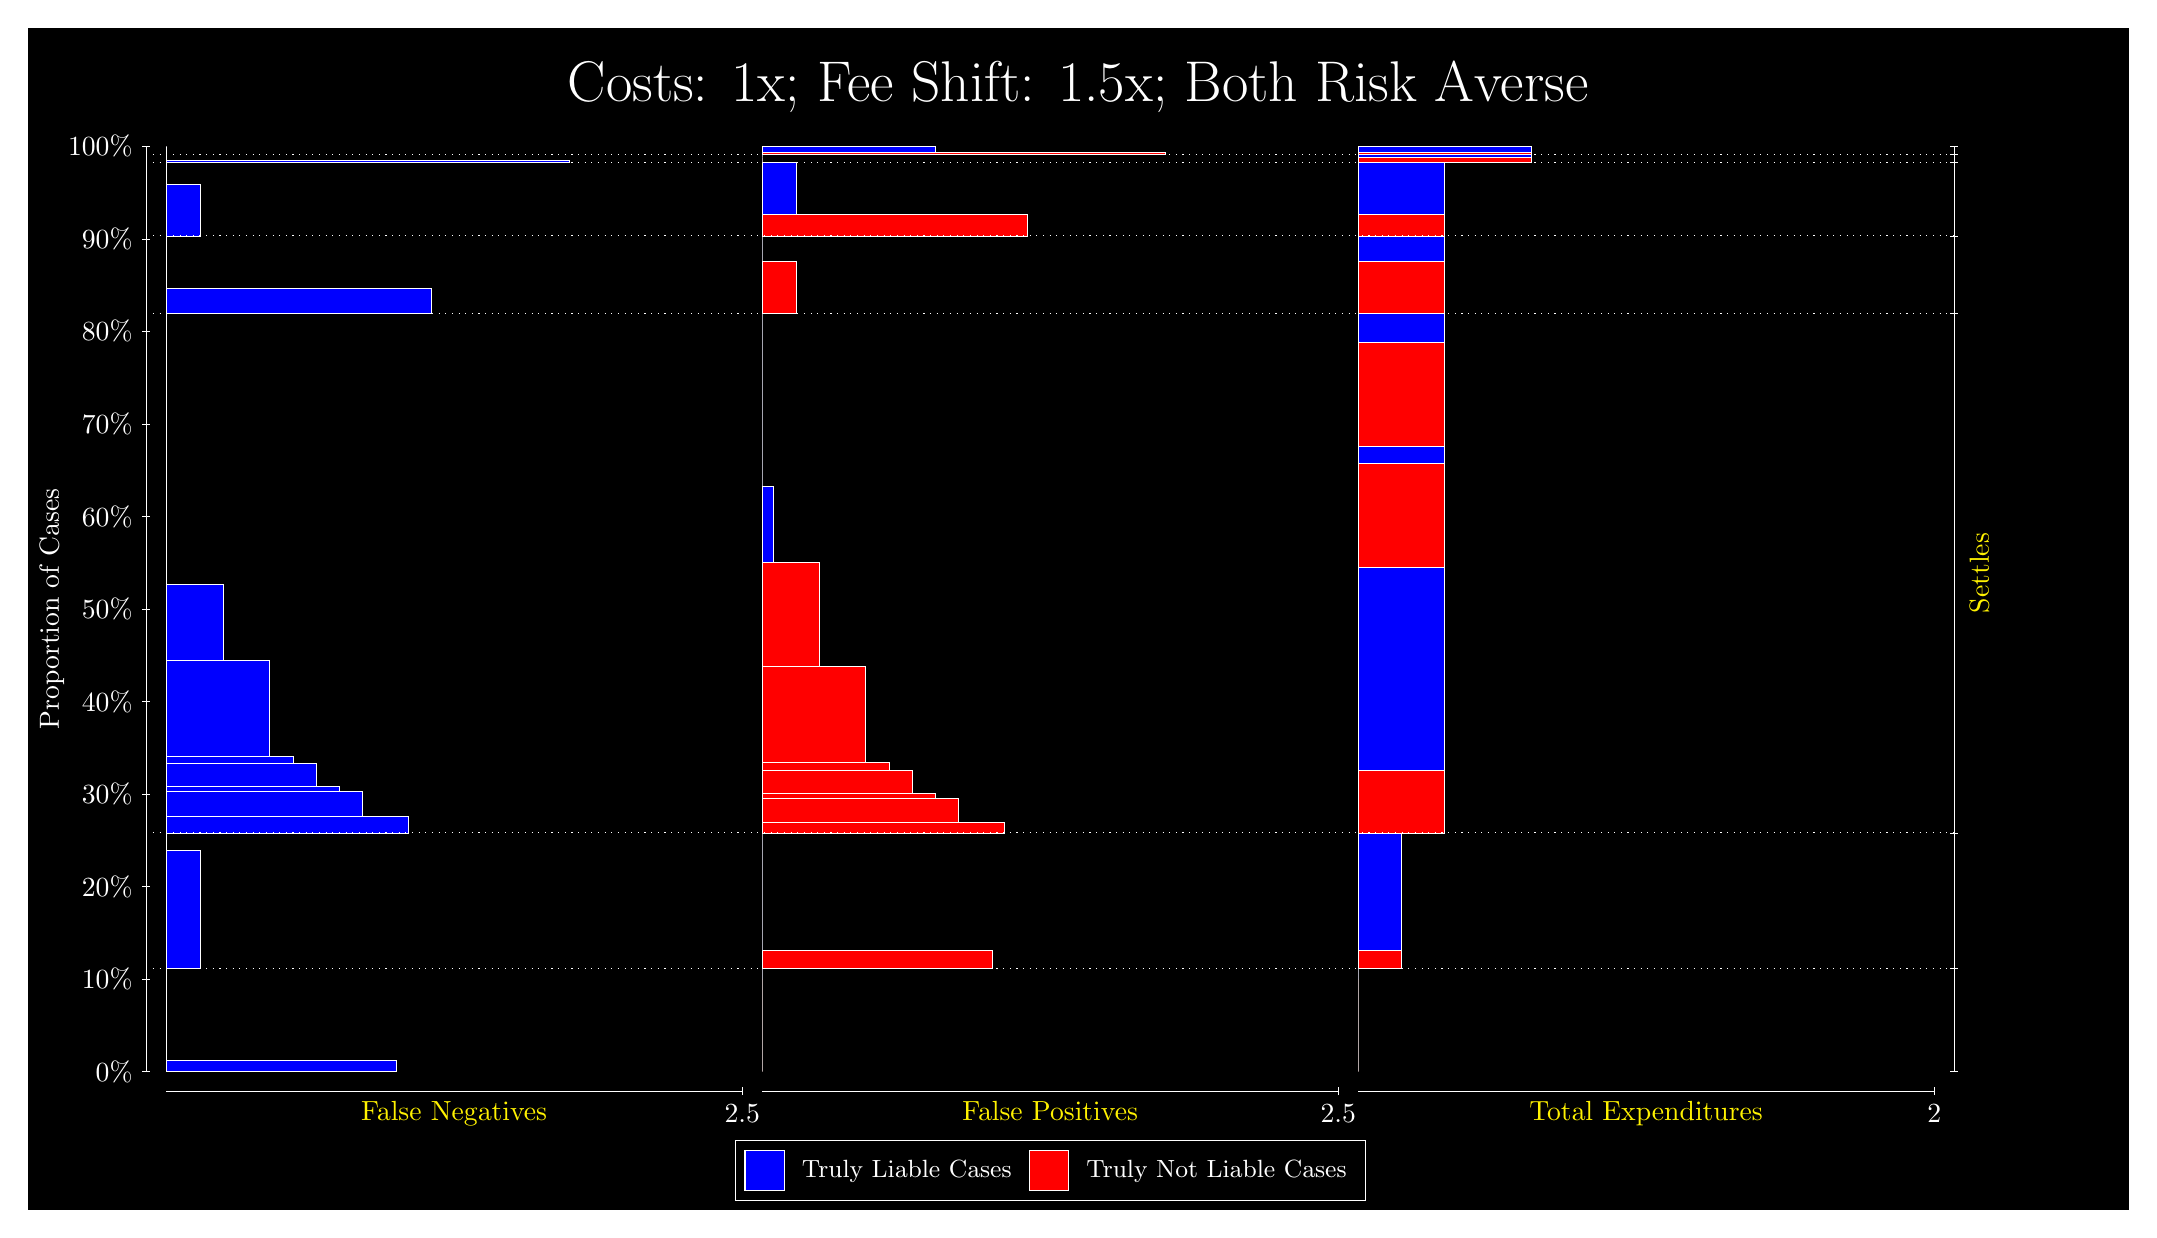
\begin{tikzpicture}
\draw[fill=black] (0,0) rectangle (26.667,15);
\draw[text=white] (0,13.5) rectangle (26.667,15) node[midway] {\huge Costs: 1x; Fee Shift: 1.5x; Both Risk Averse};
\draw[white, very thin] (1.5,1.75) -- (1.5,13.5);
\node[rotate=90, text=white, anchor=center] at (0.3, 7.625) {Proportion of Cases};
\draw[white, very thin] (1.45,1.75) -- (1.55,1.75);
\node[text=white, anchor=east] at (1.45, 1.75) {0\%};
\draw[white, very thin] (1.45,2.925) -- (1.55,2.925);
\node[text=white, anchor=east] at (1.45, 2.925) {10\%};
\draw[white, very thin] (1.45,4.1) -- (1.55,4.1);
\node[text=white, anchor=east] at (1.45, 4.1) {20\%};
\draw[white, very thin] (1.45,5.275) -- (1.55,5.275);
\node[text=white, anchor=east] at (1.45, 5.275) {30\%};
\draw[white, very thin] (1.45,6.45) -- (1.55,6.45);
\node[text=white, anchor=east] at (1.45, 6.45) {40\%};
\draw[white, very thin] (1.45,7.625) -- (1.55,7.625);
\node[text=white, anchor=east] at (1.45, 7.625) {50\%};
\draw[white, very thin] (1.45,8.8) -- (1.55,8.8);
\node[text=white, anchor=east] at (1.45, 8.8) {60\%};
\draw[white, very thin] (1.45,9.975) -- (1.55,9.975);
\node[text=white, anchor=east] at (1.45, 9.975) {70\%};
\draw[white, very thin] (1.45,11.15) -- (1.55,11.15);
\node[text=white, anchor=east] at (1.45, 11.15) {80\%};
\draw[white, very thin] (1.45,12.325) -- (1.55,12.325);
\node[text=white, anchor=east] at (1.45, 12.325) {90\%};
\draw[white, very thin] (1.45,13.5) -- (1.55,13.5);
\node[text=white, anchor=east] at (1.45, 13.5) {100\%};

\draw[white, very thin] (24.457,1.75) -- (24.457,13.5);
\draw[white, very thin] (24.407,1.75) -- (24.507,1.75);
\node[anchor=west] at (24.407, 1.75) {};
\draw[white, very thin] (24.407,3.0618) -- (24.507,3.0618);
\node[anchor=west] at (24.407, 3.0618) {};
\draw[white, very thin] (24.407,4.7803) -- (24.507,4.7803);
\node[anchor=west] at (24.407, 4.7803) {};
\draw[white, very thin] (24.407,11.379) -- (24.507,11.379);
\node[anchor=west] at (24.407, 11.379) {};
\draw[white, very thin] (24.407,12.363) -- (24.507,12.363);
\node[anchor=west] at (24.407, 12.363) {};
\draw[white, very thin] (24.407,13.294) -- (24.507,13.294);
\node[anchor=west] at (24.407, 13.294) {};
\draw[white, very thin] (24.407,13.395) -- (24.507,13.395);
\node[anchor=west] at (24.407, 13.395) {};
\draw[white, very thin] (24.407,13.5) -- (24.507,13.5);
\node[anchor=west] at (24.407, 13.5) {};

\draw[white, very thin, fill=blue] (1.75,1.75) rectangle (4.6775,1.888);
\draw[white, very thin, fill=red] (1.75,1.888) rectangle (1.75,3.0618);
\draw[white, very thin, fill=blue] (1.75,3.0618) rectangle (2.1891,4.556);
\draw[white, very thin, fill=red] (1.75,4.556) rectangle (1.75,4.7803);
\draw[white, very thin, fill=blue] (1.75,4.7803) rectangle (4.8239,4.9959);
\draw[white, very thin, fill=blue] (1.75,4.9959) rectangle (4.2384,5.303);
\draw[white, very thin, fill=blue] (1.75,5.303) rectangle (3.9457,5.3691);
\draw[white, very thin, fill=blue] (1.75,5.3691) rectangle (3.6529,5.6606);
\draw[white, very thin, fill=blue] (1.75,5.6606) rectangle (3.3602,5.7551);
\draw[white, very thin, fill=blue] (1.75,5.7551) rectangle (3.0674,6.9751);
\draw[white, very thin, fill=blue] (1.75,6.9751) rectangle (2.4819,7.9422);
\draw[white, very thin, fill=red] (1.75,7.9422) rectangle (1.75,11.379);
\draw[white, very thin, fill=blue] (1.75,11.379) rectangle (5.1167,11.698);
\draw[white, very thin, fill=red] (1.75,11.698) rectangle (1.75,12.363);
\draw[white, very thin, fill=blue] (1.75,12.363) rectangle (2.1891,13.02);
\draw[white, very thin, fill=red] (1.75,13.02) rectangle (1.75,13.294);
\draw[white, very thin, fill=blue] (1.75,13.294) rectangle (6.8732,13.329);
\draw[white, very thin, fill=red] (1.75,13.329) rectangle (1.75,13.395);
\draw[white, very thin, fill=red] (1.75,13.395) rectangle (1.75,13.43);
\draw[white, very thin, fill=blue] (1.75,13.43) rectangle (1.75,13.5);
\draw[white, very thin, fill=red] (9.3189,1.75) rectangle (9.3189,2.9238);
\draw[white, very thin, fill=blue] (9.3189,2.9238) rectangle (9.3189,3.0618);
\draw[white, very thin, fill=red] (9.3189,3.0618) rectangle (12.246,3.2861);
\draw[white, very thin, fill=blue] (9.3189,3.2861) rectangle (9.3189,4.7803);
\draw[white, very thin, fill=red] (9.3189,4.7803) rectangle (12.393,4.9141);
\draw[white, very thin, fill=red] (9.3189,4.9141) rectangle (11.807,5.2213);
\draw[white, very thin, fill=red] (9.3189,5.2213) rectangle (11.515,5.2874);
\draw[white, very thin, fill=red] (9.3189,5.2874) rectangle (11.222,5.5788);
\draw[white, very thin, fill=red] (9.3189,5.5788) rectangle (10.929,5.6734);
\draw[white, very thin, fill=red] (9.3189,5.6734) rectangle (10.636,6.8934);
\draw[white, very thin, fill=red] (9.3189,6.8934) rectangle (10.051,8.2175);
\draw[white, very thin, fill=blue] (9.3189,8.2175) rectangle (9.4652,9.1847);
\draw[white, very thin, fill=blue] (9.3189,9.1847) rectangle (9.3189,11.379);
\draw[white, very thin, fill=red] (9.3189,11.379) rectangle (9.758,12.044);
\draw[white, very thin, fill=blue] (9.3189,12.044) rectangle (9.3189,12.363);
\draw[white, very thin, fill=red] (9.3189,12.363) rectangle (12.686,12.637);
\draw[white, very thin, fill=blue] (9.3189,12.637) rectangle (9.758,13.294);
\draw[white, very thin, fill=red] (9.3189,13.294) rectangle (9.3189,13.361);
\draw[white, very thin, fill=blue] (9.3189,13.361) rectangle (9.3189,13.395);
\draw[white, very thin, fill=red] (9.3189,13.395) rectangle (14.442,13.43);
\draw[white, very thin, fill=blue] (9.3189,13.43) rectangle (11.515,13.5);
\draw[white, very thin, fill=red] (16.888,1.75) rectangle (16.888,2.9238);
\draw[white, very thin, fill=blue] (16.888,2.9238) rectangle (16.888,3.0618);
\draw[white, very thin, fill=red] (16.888,3.0618) rectangle (17.437,3.2861);
\draw[white, very thin, fill=blue] (16.888,3.2861) rectangle (17.437,4.7803);
\draw[white, very thin, fill=red] (16.888,4.7803) rectangle (17.986,5.5788);
\draw[white, very thin, fill=blue] (16.888,5.5788) rectangle (17.986,8.152);
\draw[white, very thin, fill=red] (16.888,8.152) rectangle (17.986,9.4761);
\draw[white, very thin, fill=blue] (16.888,9.4761) rectangle (17.986,9.6916);
\draw[white, very thin, fill=red] (16.888,9.6916) rectangle (17.986,11.006);
\draw[white, very thin, fill=blue] (16.888,11.006) rectangle (17.986,11.379);
\draw[white, very thin, fill=red] (16.888,11.379) rectangle (17.986,12.044);
\draw[white, very thin, fill=blue] (16.888,12.044) rectangle (17.986,12.363);
\draw[white, very thin, fill=red] (16.888,12.363) rectangle (17.986,12.637);
\draw[white, very thin, fill=blue] (16.888,12.637) rectangle (17.986,13.294);
\draw[white, very thin, fill=red] (16.888,13.294) rectangle (19.083,13.361);
\draw[white, very thin, fill=blue] (16.888,13.361) rectangle (19.083,13.395);
\draw[white, very thin, fill=red] (16.888,13.395) rectangle (19.083,13.43);
\draw[white, very thin, fill=blue] (16.888,13.43) rectangle (19.083,13.5);
\draw[white, dotted] (1.5,3.0618) -- (24.457,3.0618);
\draw[white, dotted] (1.5,4.7803) -- (24.457,4.7803);
\draw[white, dotted] (1.5,11.379) -- (24.457,11.379);
\draw[white, dotted] (1.5,12.363) -- (24.457,12.363);
\draw[white, dotted] (1.5,13.294) -- (24.457,13.294);
\draw[white, dotted] (1.5,13.395) -- (24.457,13.395);
\draw[white, very thin] (1.75,1.5) -- (9.0689,1.5);
\node[text=yellow, anchor=north] at (5.4094, 1.5) {False Negatives};
\draw[white, very thin] (9.0689,1.45) -- (9.0689,1.55);
\node[text=white, anchor=north] at (9.0689, 1.45) {2.5};

\draw[white, very thin] (9.3189,1.5) -- (16.638,1.5);
\node[text=yellow, anchor=north] at (12.978, 1.5) {False Positives};
\draw[white, very thin] (16.638,1.45) -- (16.638,1.55);
\node[text=white, anchor=north] at (16.638, 1.45) {2.5};

\draw[white, very thin] (16.888,1.5) -- (24.207,1.5);
\node[text=yellow, anchor=north] at (20.547, 1.5) {Total Expenditures};
\draw[white, very thin] (24.207,1.45) -- (24.207,1.55);
\node[text=white, anchor=north] at (24.207, 1.45) {2};



\node[text=yellow, centered, rotate=90] at (24.777, 8.0799) {Settles};





\draw (12.978300999999998,1.5) node[draw=none] (baseCoordinate) {};
\begin{scope}[align=center]
        \matrix[scale=0.5, draw=white, below=0.5cm of baseCoordinate, nodes={draw}, column sep=0.1cm]{
            \node[rectangle, draw, minimum width=0.5cm, minimum height=0.5cm, fill=blue] {}; &
            \node[draw=none, font=\small, text=white] (B) {Truly Liable Cases}; &
            \node[rectangle, draw, minimum width=0.5cm, minimum height=0.5cm, fill=red] {}; &
            \node[draw=none, font=\small, text=white] (B) {Truly Not Liable Cases}; \\
            };
\end{scope}

\end{tikzpicture}
\end{document}